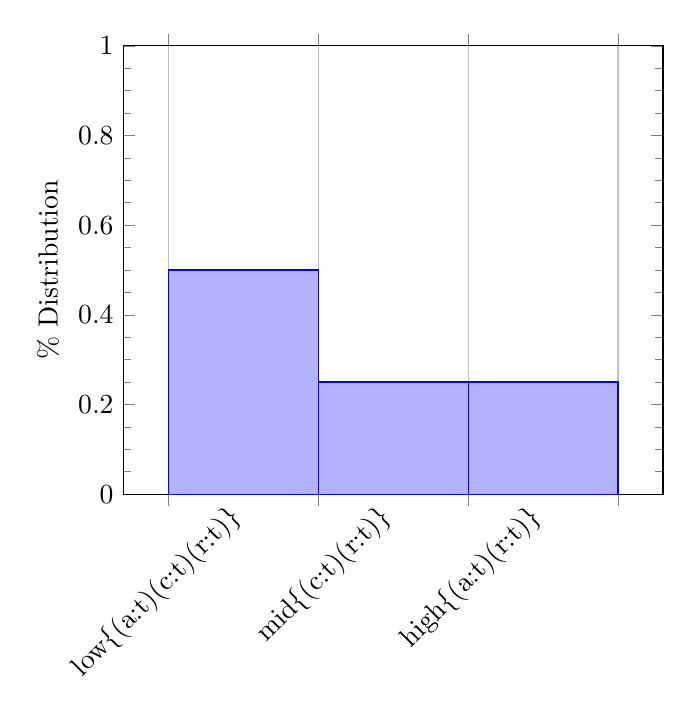
\begin{tikzpicture}
	\begin{axis}[
	ybar interval, 
	ymax=1,ymin=0, 
	minor y tick num = 3,
	ylabel = {\% Distribution},
	symbolic x coords={low\{(a:t)(c:t)(r:t)\}, mid\{(c:t)(r:t)\}, high\{(a:t)(r:t)\}, high\{(y:t)(r:t)\}},
	x tick label style={font=\normalsize, rotate=45, anchor=east},
	]
	\addplot coordinates {(low\{(a:t)(c:t)(r:t)\}, 0.5) (mid\{(c:t)(r:t)\}, 0.25) (high\{(a:t)(r:t)\}, 0.25) (high\{(y:t)(r:t)\}, 0.10)};
	\end{axis}
\end{tikzpicture}

%\begin{tikzpicture}

%\definecolor{bblue}{HTML}{4F81BD}

%\begin{axis}[
%major x tick style = transparent,
%ymin=0,
%bar width=1cm,
%minor y tick num = 3,
%ymajorgrids = true,
%ylabel = {\% distribution},
%symbolic x coords={low\{(a:t)(c:t)(r:t)\}, mid\{(c:t)(r:t)\}, high\{(a:t)(r:t)\}},
%xtick = data,
%x tick label style={font=\normalsize, rotate=45, anchor=east},
%]
%\addplot[ybar , style={bblue,fill=bblue,mark=none}]
%coordinates {(low\{(a:t)(c:t)(r:t)\}, 0.5) (mid\{(c:t)(r:t)\}, 0.25) (high\{(a:t)(r:t)\}, 0.25)};

%\end{axis}
%\end{tikzpicture}